\chapter{Methodology}
\section{Thin Film Fabrication}
Thirty glass substrates, measuring $1"\times0.25"$, were cut from microscope slides.
These substrates were subject to three successive ionic layer adhesion and reaction (SILAR) processes, S1, S2, and S3, as will be detailed in this section.
All of the SILAR processes consist of a certain number of deposition cycles from a fixed precursor solution with $0.095M$ Zn$^{2+}$ and $0.190M$ NaOH and a thermal annealing at certain temperatures \cite{florido17, gao08}.

Table \ref{tab:processes} summarizes the different SILAR processes along with the variations in processing parameters.

\begin{table}
  \caption{Processing parameters manipulated and SILAR processes}
  \centering
  \begin{tabular}{c c c c}
    \hline\hline
    --- & S1 & S2 & S3 \\
    \hline
    Depostion cycles & 100 & 75 & 100 \\
    Annealing temperature & 450$\degg$ & 450$\degg$ & 500$\degg$ \\[1ex]
    \hline
  \end{tabular}
  \label{tab:processes}
\end{table}

\section{Thin Film Characterization}
The fabricated thin films were characterized for determination of thin film structure and properties.

One thin film fabricated using each of the fabrication processes was chosen for optical microscopy.
The fabricated material was split into four sections as shown in Figure \ref{fig:orient}.
The sections were chosen such that the four corners of the rectangular substrate represent different probe volumes.
The thin films were viewed under the high power objective lens ($400\times$) of a digital compound microscope.

\begin{figure}
  \centering
  \begin{tabular}{| c | c |}
    \hline
    1 & 3 \\
    \hline
    2 & 4 \\[0.5ex]
    \hline
  \end{tabular}
  \caption{Basic orientation matrix}
  \label{fig:orient}
\end{figure}

Overall thin film structure were also characterized with x-ray diffraction, using Cu-K$\alpha$ anode ($\lambda = \SI{1.54}{\angstrom}$), and scanning electron microscopy at $\SI{20}{\kilo\V}$.

Finally, the thin films sheet resistance values were derived from measurements from four-point probe sensing.
The schematic for the four-point probe mechanism are shown in Figure \ref{fig:fpt}.

\begin{figure}
  \centering
  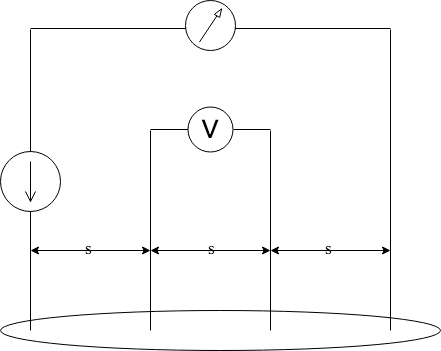
\includegraphics[scale=0.3]{FourPoint}
  \caption{Four point probe mechanism for determination of sheet resistance}
  \label{fig:fpt}
\end{figure}

\section{Model Creation}
\subsection{Definition of microstructure functions}
There are a total of 20 discrete microstructure functions (DMF) that are studied for the study.
The definitions are divided into four categories depending on which of two axes will the DMFs be assumed to be periodic in.
Each of the four categories contains five DMFs, which differ based on the method for determining the number of discrete local states within a certain probe volume $V$.

The functions can be summarized as Table \ref{tab:fxns}.
The dimensions of the probe volume $V$ were chosen as odd products of small primes (2, 3, 5, and 7) to aid in the computation of two point spatial correlations, as will be discussed in the following subsection, with the exception of one function, with accounts for the dimensions of the size of a high resolution digital image.

\begin{table}
  \caption{Summary of discrete microstructure functions}
  \centering
  \begin{tabular}{c c c}
    \hline\hline
    Periodic axes & Local states & Size of $V$ \\
    \hline
    Both $i, j$ & Two & $225 \times 225$ \\
    Both $i, j$ & Two & $441 \times 441$ \\
    Both $i, j$ & Three & $225 \times 225$ \\
    Both $i, j$ & Three & $441 \times 441$ \\
    Both $i, j$ & Three & $1920 \times 1080$ \\
    \hline
    $j$ & Two & $225 \times 225$ \\
    $j$ & Two & $441 \times 441$ \\
    $j$ & Three & $225 \times 225$ \\
    $j$ & Three & $441 \times 441$ \\
    $j$ & Three & $1920 \times 1080$ \\
    \hline
    $i$ & Two & $225 \times 225$ \\
    $i$ & Two & $441 \times 441$ \\
    $i$ & Three & $225 \times 225$ \\
    $i$ & Three & $441 \times 441$ \\
    $i$ & Three & $1920 \times 1080$ \\
    \hline
    None & Two & $225 \times 225$ \\
    None & Two & $441 \times 441$ \\
    None & Three & $225 \times 225$ \\
    None & Three & $441 \times 441$ \\
    None & Three & $1920 \times 1080$ \\[1ex]
  \end{tabular}
  \label{tab:fxns}
\end{table}

\subsection{Calculation of two-point spatial correlations}
Two point spatial correlations are derived from optical microscopy images through the definition of the measures \cite{gupta15}.

\[
  m^{np}_r = \dfrac{1}{S_rN} \sum_{i=0}^{N} \sum_{i=0}^{R} m^p_r m^n_r
\]

where $n, p$ are the discrete local states of interest and $r$ is the spatial bin of interest.

Image data were transformed into Julia 2D arrays \cite{julia15} and further into a user defined data structure named \emph{MaterialImage} which accounts for the parameters used for defining the DMFs (from the previous subsection).
There are a total of 20 sets two point spatial correlations that will be considered.

\subsection{Determination of optimal film orientation}
Since the preferred orientation of the fabrication of thin films is unknown, each of the three thin films have four hypothesized orientations based on circular permuations of the orientation matrix (Figure \ref{fig:orient}).

For each of the calculated two point spatial correlations, the values will undergo principal component analysis to obtain the orthogonal latent descriptors \cite{gupta15, sun17}.
This is done with \emph{MultivariateStats.jl}, a package available for multivariate statistical analysis \cite{mvstats}.
Optimal orientation is determined when the variance of the dimensionally-reduced two point statistics, \textit{i.e. the matrix trace of the covariance matrix} is minimized.

\subsection{Determination of optimal microstructure function}
The plots for the two-point statistics are manually compared.
Partial least squares analysis (PLSA) is done to compare the ability of the DMF to capture the variation of derived sheet resistance values.
Evaluation of the optimal microstructure function will be based on the following parameters:

\begin{enumerate}
  \item Variance capture via PLSA
  \item Qualitative assessment of clustering of microstructure ensembles
\end{enumerate}
